\begin{figure}[H]
     \begin{subfigure}[h]{0.23\textwidth}
         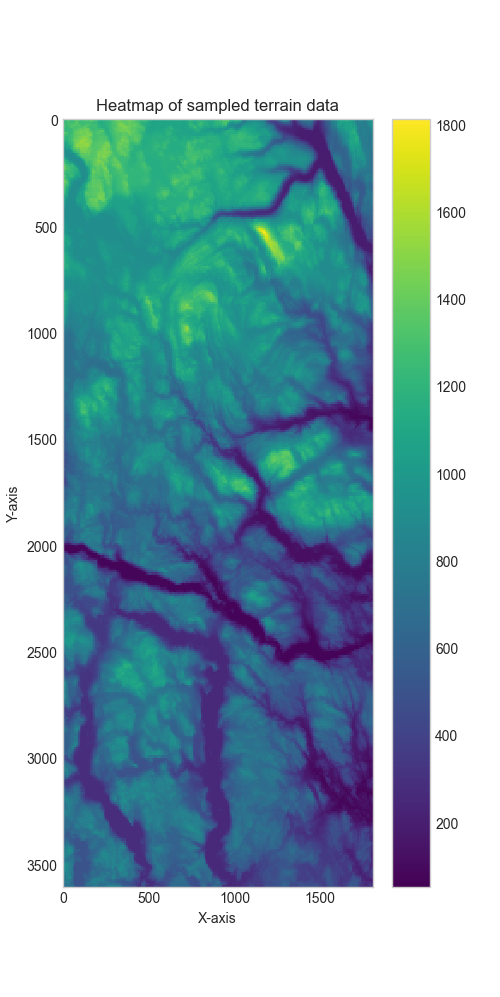
\includegraphics[width=\textwidth]{Images/sampled_data_heatmap.png}
         \caption{Original sampled data}
         \label{terrain data heatmap}
     \end{subfigure}
     \hfill
     \begin{subfigure}[h]{0.23\textwidth}
         \centering
         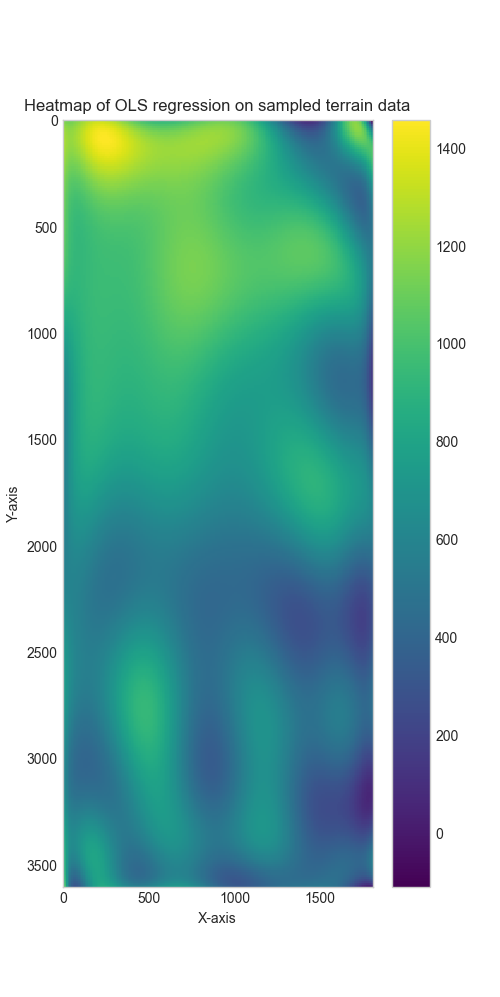
\includegraphics[width=\textwidth]{Images/ols_terrain_heatmap.png}
         \caption{Ordinary least squares}
         \label{fig:ols heatmap}
     \end{subfigure}
     \hfill
     \begin{subfigure}[h]{0.23\textwidth}
         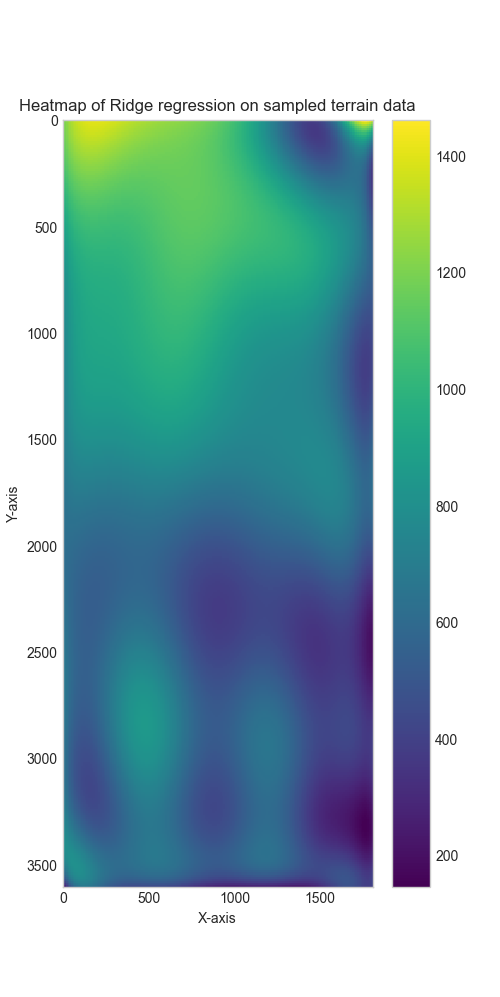
\includegraphics[width=\textwidth]{Images/ridge_terrain_heatmap.png}
         \caption{Ridge}
         \label{fig:ridge heatmap}
     \end{subfigure}
     \hfill
     \begin{subfigure}[h]{0.23\textwidth}
         \centering
         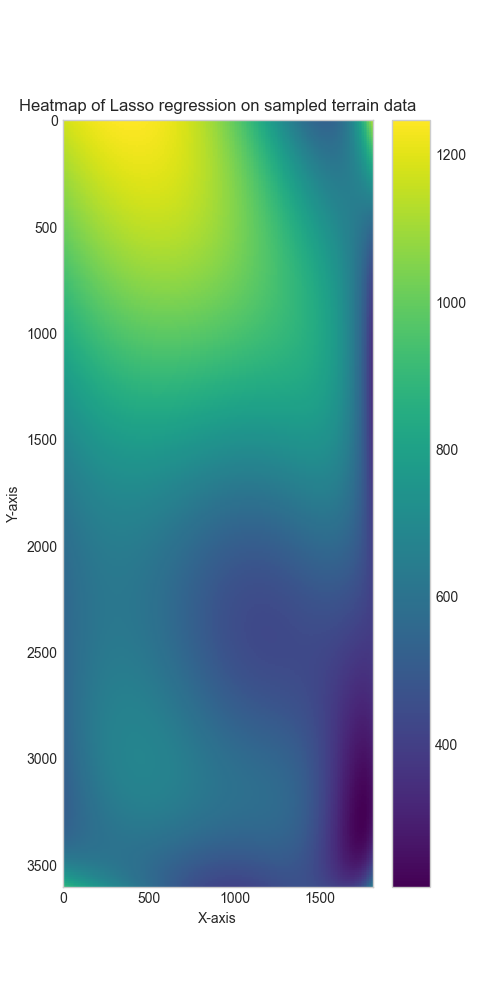
\includegraphics[width=\textwidth]{Images/lasso_terrain_heatmap.png}
         \caption{Lasso}
         \label{fig:lasso heatmap}
     \end{subfigure}
        \caption{Heatmaps showing the true terrain side by side with the estimated terrain of OLS, Ridge and Lasso without cross validation. We see that the predictions is most precise with OLS, less precise with Ridge, and most blurry with Lasso.}
        \label{fig:four graphs}
\end{figure}


When plotting our results in figure \ref{fig:lasso heatmap}, found in appendix A, in a heatmap, we see that it is able to reproduce some of the structures in the original data, but the result is blurry compared to that of Ridge and OLS. 